\section{Perceptron}

In the 1940s, computers were already excelling at executing tasks with precision and performing arithmetic operations at remarkable speeds. 
However, researchers aspired for more than mere computational efficiency. 
They envisioned machines capable of handling noisy data, interacting directly with their environment, operating in a massively parallel and fault-tolerant manner, and adapting to dynamic circumstances.
Their ambition led to the quest for a new computational model

\paragraph*{Human neurons}
The human brain consists of an enormous network of computing units, with each neuron connected to many others through synapses. 
Information transmission in the brain relies on chemical processes: dendrites gather signals from synapses, which can either excite or inhibit the neuron. 
When the cumulative signal surpasses a certain threshold, the neuron fires, releasing an electrical charge.

This biological computational model is marked by its distributed nature, fault-tolerant redundancy, and inherent parallelism. 
The Perceptron, inspired by these principles, became one of the first attempts to emulate the brain's computational capabilities.

\subsection{Perceptron}
In the mid-20th century, researchers explored various models of the brain. 
In 1943, Warren McCulloch and Walter Pitts proposed the threshold logic unit, where the activation function operated as a threshold unit. 
Later, in 1957, Frank Rosenblatt introduced the first Perceptron, featuring weights encoded in potentiometers and electric motors for weight adjustments during learning. 
By 1960, Bernard Widrow introduced a critical improvement: the inclusion of a bias term to represent the threshold value.

\begin{figure}[H]
    \centering
    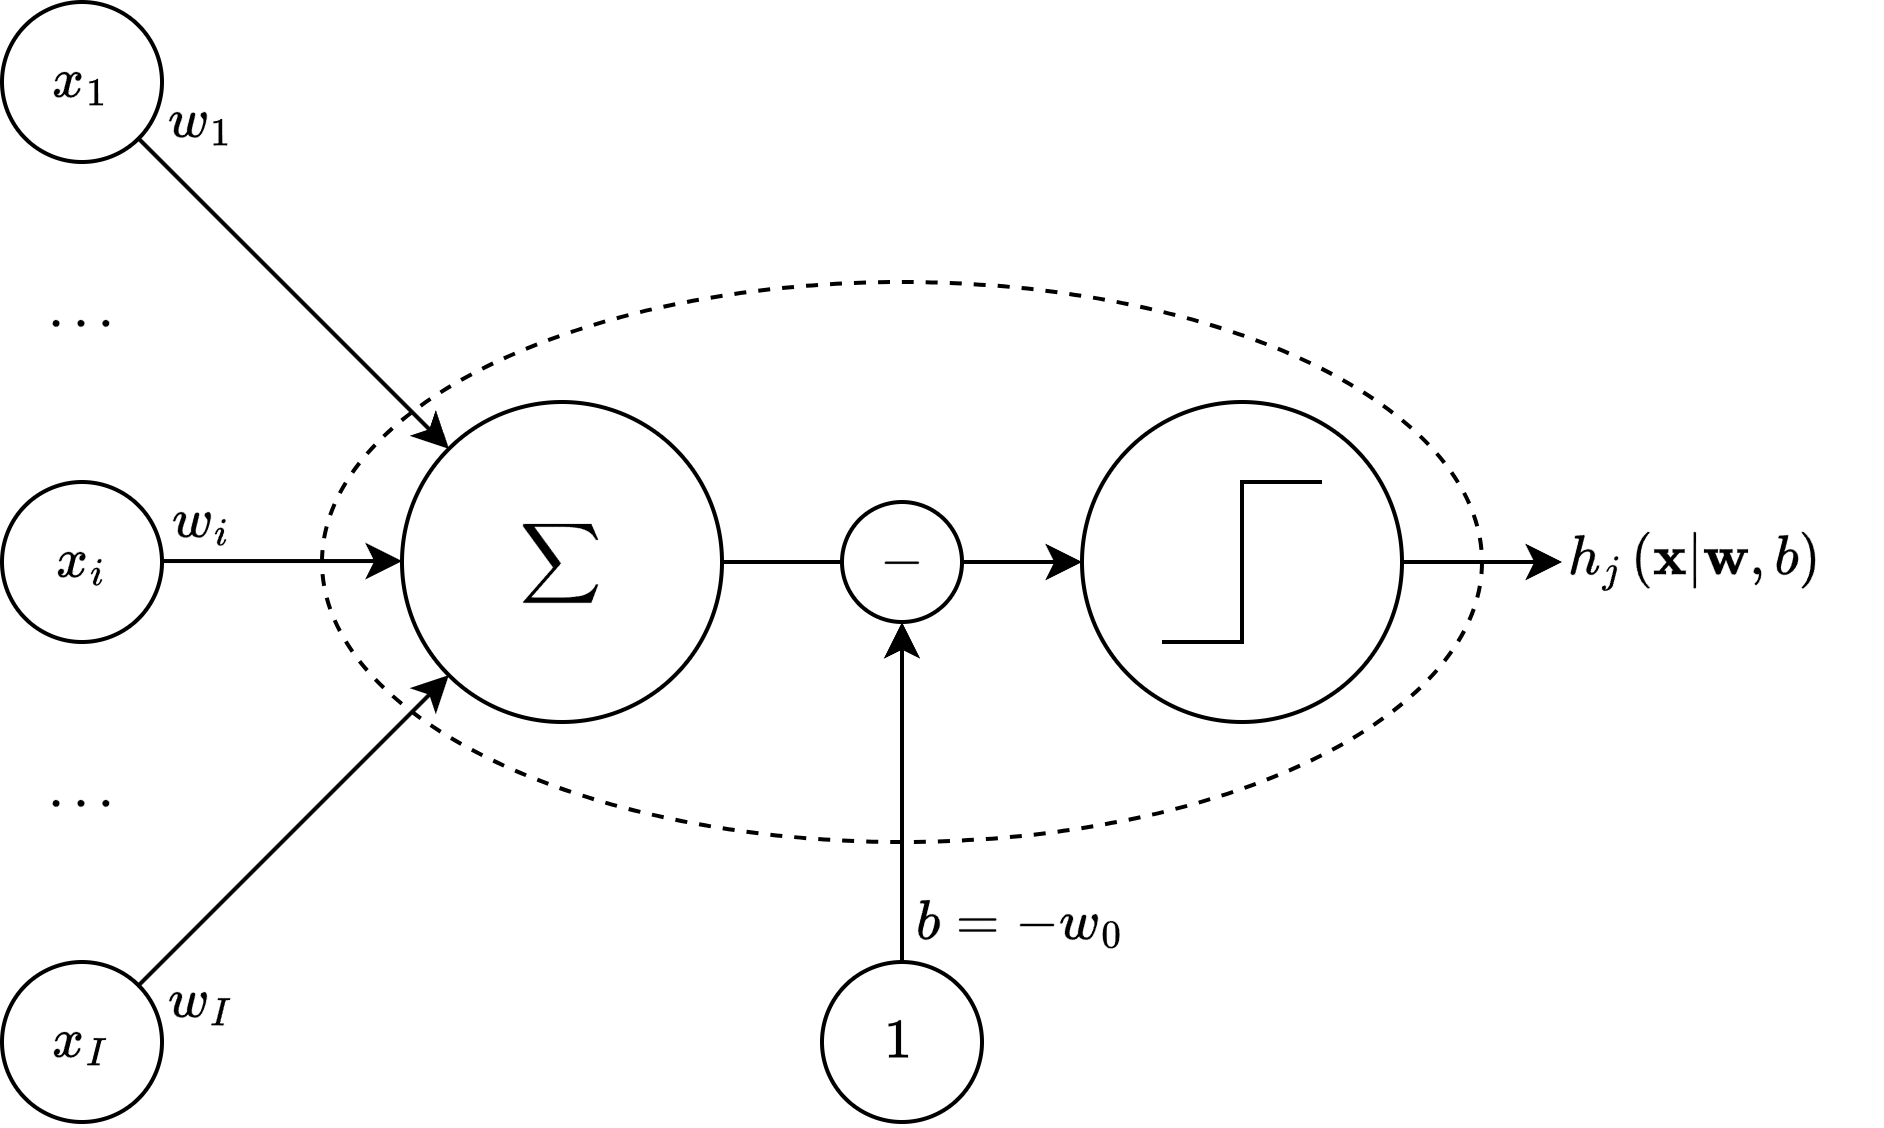
\includegraphics[width=0.75\linewidth]{images/neuron.png}
    \caption{Perceptron}
\end{figure}
\noindent The output function $h_j(\mathbf{x}\mid\mathbf{w},b)$ is given by:
\[h_j(\mathbf{x}\mid\mathbf{w},b)=h_j\left(\sum_{i=1}^Iw_ix_i-b\right)=h_j\left(\sum_{i=0}^Iw_ix_i\right)=h_j\left(\mathbf{w}^T\mathbf{x}\right)\]
\noindent The activation function in an artificial neuron can take various forms.
The Perceptron computes a weighted sum of its inputs and applies a thresholding function to produce its output:
\[h_j(\mathbf{x}\mid\mathbf{w})=h_j\left(\mathbf{w}^T\mathbf{x}\right)=\text{sign}(\mathbf{w}^T\mathbf{x})\]
This defines a linear classifier, where the decision boundary is a hyperplane described by:
\[\mathbf{w}^T\mathbf{x}=0\]
The linear decision boundary enables the Perceptron to implement Boolean logic operators. 
However, the Perceptron struggles when data cannot be separated by a linear boundary.
In such cases, additional strategies are necessary. 
These challenges paved the way for more advanced models, such as Multi-Layer Perceptrons.

\paragraph*{Hebbian learning}
Hebbian learning, often summarized by the phrase cells that fire together, wire together, follows these principles:
\begin{enumerate}
    \item Initialize weights randomly.
    \item Adjust weights for each sample, but only if the sample is misclassified.
\end{enumerate}
The weight update rule is given by:
\[\mathbf{w}_i^{(k+1)}=\mathbf{w}_i^{(k)}+\eta \mathbf{x}_i^{(k)}t^{(k)}\]
Here, $\eta$ is the learning rate, $\mathbf{x}_i^{(k)}$ represents the $i$-th input to the Perceptron at time $k$, and $t^{(k)}$ is the desired output at the same time. 